% =====================================================================
%  How Our Landing-Site Algorithm Works
%  NASA Space Apps Challenge 2026 -- team design document
%  Compile on Overleaf with pdfLaTeX (default). Single file, no images.
% =====================================================================
\documentclass[11pt,a4paper]{article}

\usepackage[margin=2.5cm]{geometry}
\usepackage{tikz}
\usetikzlibrary{arrows.meta, positioning, calc, fit}
\usepackage{booktabs, tabularx, array}
\usepackage{amsmath}
\usepackage{algorithm}
\usepackage{algpseudocode}
\usepackage{float}
\usepackage{enumitem}
\usepackage{xurl}
\usepackage[hidelinks]{hyperref}

\setlist{itemsep=2pt, topsep=4pt}
\setlength{\parskip}{4pt}
\newcolumntype{Y}{>{\raggedright\arraybackslash}X}
\newcommand{\sun}{\odot}
\newcommand{\earth}{\oplus}

\title{How Our Landing-Site Algorithm Works\\[4pt]
\large Step-by-step design for the team\\
NASA Space Apps Challenge 2026: Lunar Landing-Site Challenge}
\author{Ash\\Princess Sumaya University for Technology}
\date{October 2026}

\begin{document}
\maketitle

% ---------------------------------------------------------------------
\section{What the Algorithm Is Based On}

We do not invent the science. The algorithm combines three things that already exist:

\begin{enumerate}
  \item \textbf{Physics.} Sunlight and radio travel in straight lines, and the Moon has no atmosphere to bend them. So ``can this spot see the Sun?'' is exactly ``does the straight line from here to the Sun hit any terrain?''
  \item \textbf{NASA's measured data.} Terrain heights come from the LOLA laser altimeter on the Lunar Reconnaissance Orbiter. Sun and Earth positions for any hour come from JPL's ephemerides through the SPICE toolkit~\cite{spice}.
  \item \textbf{NASA's requirements.} They define what ``good'' means: land within 6\textdegree{} of the pole, slope under 10\textdegree{} over 100\,m, direct line of sight to Earth with no relay, and enough sunlight~\cite{nasa-artemis}.
\end{enumerate}

NASA scientists use this same ``horizon method'' to publish long-term illumination and Earth-visibility maps of the poles~\cite{pgda}. That proves the method is sound and gives us data to check against (Step~5). Figure~\ref{fig:pipeline} shows the full pipeline.

\begin{figure}[ht]
\centering
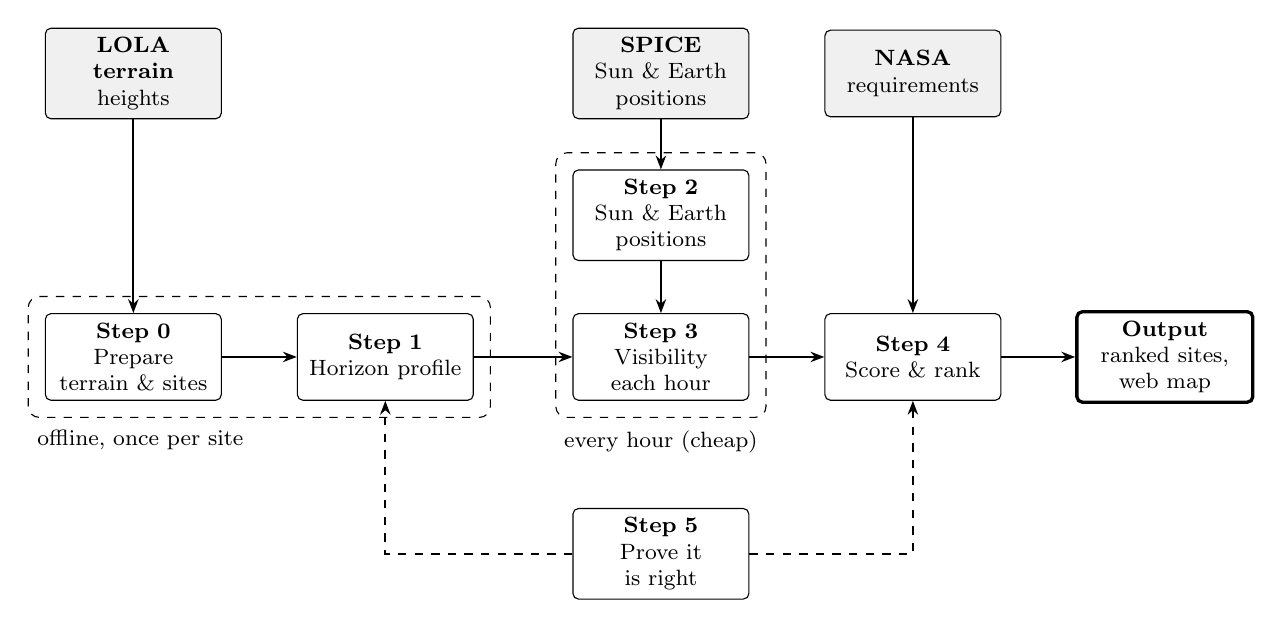
\begin{tikzpicture}[font=\footnotesize,
  box/.style={draw, rounded corners=2pt, text width=2.0cm, align=center, minimum height=1.1cm},
  inp/.style={box, fill=gray!12},
  arr/.style={thick, -{Stealth[length=5pt]}},
  grp/.style={draw, dashed, rounded corners=4pt, inner sep=6pt}]
  \node[inp] (lola)  at (1.2,3.6)  {\textbf{LOLA terrain}\\heights};
  \node[inp] (spice) at (7.9,3.6)  {\textbf{SPICE}\\Sun \& Earth positions};
  \node[inp] (req)   at (11.1,3.6) {\textbf{NASA}\\requirements};
  \node[box] (s0) at (1.2,0)  {\textbf{Step 0}\\Prepare terrain \& sites};
  \node[box] (s1) at (4.4,0)  {\textbf{Step 1}\\Horizon profile};
  \node[box] (s2) at (7.9,1.8) {\textbf{Step 2}\\Sun \& Earth positions};
  \node[box] (s3) at (7.9,0)  {\textbf{Step 3}\\Visibility each hour};
  \node[box] (s4) at (11.1,0) {\textbf{Step 4}\\Score \& rank};
  \node[box, very thick] (out) at (14.3,0) {\textbf{Output}\\ranked sites, web map};
  \node[box] (s5) at (7.9,-2.5) {\textbf{Step 5}\\Prove it is right};
  \node[grp, fit=(s0)(s1)] (g1) {};
  \node[grp, fit=(s2)(s3)] (g2) {};
  \node[below right=1pt and 0pt of g1.south west] {offline, once per site};
  \node[below=1pt of g2.south] {every hour (cheap)};
  \draw[arr] (lola) -- (s0);
  \draw[arr] (s0) -- (s1);
  \draw[arr] (s1) -- (s3);
  \draw[arr] (spice) -- (s2);
  \draw[arr] (s2) -- (s3);
  \draw[arr] (s3) -- (s4);
  \draw[arr] (req) -- (s4);
  \draw[arr] (s4) -- (out);
  \draw[arr, dashed] (s5.west) -| (s1.south);
  \draw[arr, dashed] (s5.east) -| (s4.south);
\end{tikzpicture}
\caption{The pipeline. Shaded boxes are inputs from NASA. Steps 0--1 run once, offline; Steps 2--3 are a fast lookup for any dates the user picks. Step 5 checks the results of Steps 1 and 4.}
\label{fig:pipeline}
\end{figure}

% ---------------------------------------------------------------------
\section{Step 0: Prepare the Terrain and Candidate Sites}

\begin{itemize}
  \item \textbf{Get the terrain.} Download two LOLA south-pole elevation maps~\cite{lola}: one with 20\,m pixels for the terrain near each site, and one with 240\,m pixels for distant terrain. Step~1 explains why both are needed.
  \item \textbf{Crop with a margin.} Candidate sites lie within 6\textdegree{} of the pole, but Step~1 looks far beyond each site. The 240\,m map must therefore reach the maximum look-out distance $D_{\max} = 250$\,km beyond every site, and the 20\,m map must reach 40\,km beyond every site.
  \item \textbf{Fix the coordinates.} Both maps use the same polar-stereographic projection. A site is given by its map position $x, y$ in metres, plus its lat/lon. A pixel (row, column) is not a unique address, because the two maps have different pixel sizes.
  \item \textbf{Slope gate.} Compute the slope over a 100\,m baseline and drop every site at 10\textdegree{} or steeper.
  \item \textbf{Candidate grid.} Start with every $k$-th pixel, then refine around the best areas. NASA's published average illumination map~\cite{pgda} can pre-select promising areas so we do not waste time on permanently dark craters.
\end{itemize}

\textbf{Direction convention (critical).} At the south pole every direction is ``north'', so compass bearings do not work. All steps measure azimuth $\theta$ from the map's $+x$ axis, counterclockwise, 0--360\textdegree. Longitude 0 is map up ($\theta = 90^\circ$), so Earth always sits near $\theta = 90^\circ$. Steps 1 and 2 must use exactly this convention.

% ---------------------------------------------------------------------
\section{Step 1: Horizon Profile (the Hardest Step)}

Stand at a site and look in direction $\theta$. Walk outward over the terrain. At each distance $d$, compute the angle up to the terrain. The steepest angle found is the horizon $H(\theta)$ in that direction (Figure~\ref{fig:cross}). Repeat for 1{,}440 directions, 0.25\textdegree{} apart, to get the site's full skyline.

\begin{equation}
H(\theta) = \max_{d \le D_{\max}} \operatorname{atan2}\!\Big( (R+z)\cos\varphi - (R+h_0+m),\; (R+z)\sin\varphi \Big),
\qquad \varphi = d/R
\label{eq:horizon}
\end{equation}

Here $z(d)$ is the terrain height at distance $d$ (interpolated between pixels), $h_0$ is the site height, $m$ is the mast height, $R = 1737.4$\,km is the Moon's radius, and $\varphi$ is the angle between the site and the terrain point, seen from the Moon's centre. The formula is exact on a sphere. For intuition, it is almost the same as $\arctan\!\big((z - h_0 - m - d^2/2R)/d\big)$, where $d^2/2R$ is how far the Moon's curved surface drops below a flat line. The curvature matters: at 20\,km the drop is about 115\,m, which shifts the angle by about 0.3\textdegree. That is significant when the Sun is only about 1.5\textdegree{} up.

\textbf{Two terrain maps.} Within 40\,km of the site the walk samples the 20\,m map; beyond that it samples the 240\,m map. The near field decides more than it seems. On the 240\,m map alone, our test site on Shackleton's rim looks sunlit about 87\% of the time. On 20\,m terrain, the same site seen from a 2\,m mast is almost always dark (0.3\%), because a crest 103\,m away and 9.5\,m higher blocks the Sun. A 10\,m mast lifts it back to about 80\%. The 240\,m map had smoothed that crest away.

\begin{figure}[ht]
\centering
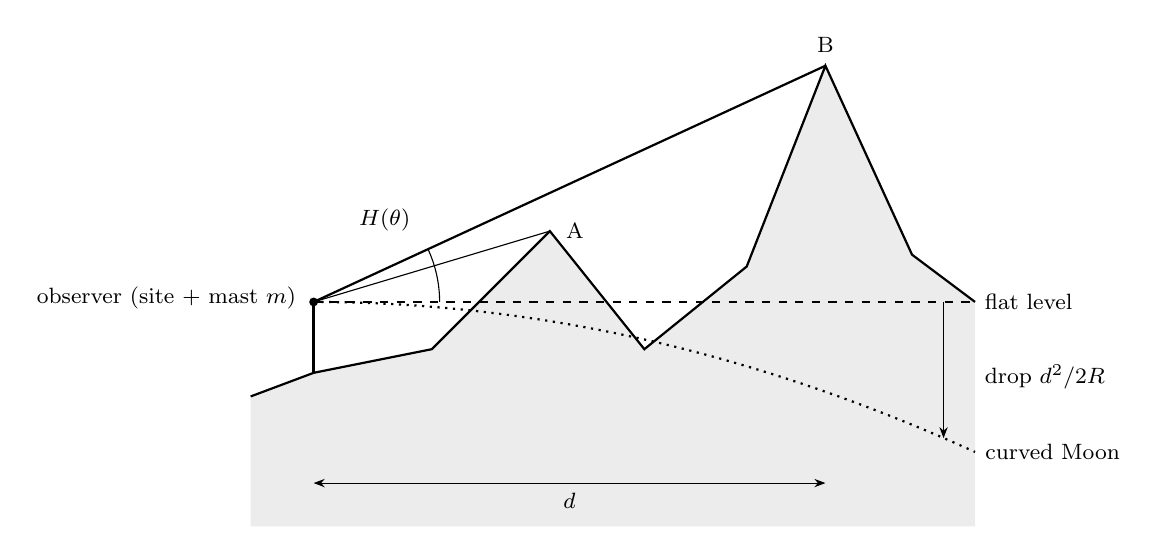
\begin{tikzpicture}[font=\footnotesize]
  \fill[gray!15] (-0.8,-0.3) -- (0,0) -- (1.5,0.3) -- (3,1.8) -- (4.2,0.3) -- (5.5,1.35) -- (6.5,3.9) -- (7.6,1.5) -- (8.4,0.9) -- (8.4,-1.95) -- (-0.8,-1.95) -- cycle;
  \draw[thick] (-0.8,-0.3) -- (0,0) -- (1.5,0.3) -- (3,1.8) -- (4.2,0.3) -- (5.5,1.35) -- (6.5,3.9) -- (7.6,1.5) -- (8.4,0.9);
  \draw[very thick] (0,0) -- (0,0.9);
  \fill (0,0.9) circle (1.6pt);
  \node[left] at (-0.1,0.95) {observer (site + mast $m$)};
  \draw[dashed] (0,0.9) -- (8.4,0.9) node[right] {flat level};
  \draw[dotted, thick, domain=0:8.4, samples=40] plot (\x, {0.9-0.027*\x*\x}) node[right] {curved Moon};
  \draw[-{Stealth[length=4pt]}] (8.0,0.9) -- (8.0,-0.83);
  \node[right] at (8.4,-0.05) {drop $d^2/2R$};
  \draw (0,0.9) -- (3,1.8);
  \draw[thick] (0,0.9) -- (6.5,3.9);
  \node at (3.32,1.8) {A};
  \node[above] at (6.5,3.95) {B};
  \draw (1.6,0.9) arc (0:24.78:1.6);
  \node[above left] at (1.35,1.68) {$H(\theta)$};
  \draw[{Stealth[length=4pt]}-{Stealth[length=4pt]}] (0,-1.4) -- node[below] {$d$} (6.5,-1.4);
\end{tikzpicture}
\caption{Step 1 in one direction. Keep the steepest angle to the terrain. Peak A is nearer; peak B is farther but higher, and it sets the horizon because its angle is larger. Heights and curvature are exaggerated.}
\label{fig:cross}
\end{figure}

\begin{algorithm}[ht]
\caption{Horizon profile for one site}
\begin{algorithmic}[1]
\Require terrain $Z$, site $(x_0, y_0)$, height $h_0$, mast $m$, look-out distance $D_{\max}$
\For{$\theta = 0^\circ, 0.25^\circ, \dots, 359.75^\circ$}
  \State $H[\theta] \gets -90^\circ$;\quad $d \gets d_{\min}$
  \While{$d \le D_{\max}$}
    \State $(x, y) \gets (x_0 + d\cos\theta,\; y_0 + d\sin\theta)$
    \State $z \gets \Call{Interpolate}{Z, x, y}$ \Comment{20\,m map within 40\,km, 240\,m beyond}
    \State $\alpha \gets$ angle to $(d, z)$ from Equation~\eqref{eq:horizon}
    \State $H[\theta] \gets \max(H[\theta], \alpha)$
    \State $d \gets d + \Call{Step}{d}$ \Comment{$\max(\text{pixel}/2,\ 0.002\,d)$}
  \EndWhile
\EndFor
\State \Return $H$
\end{algorithmic}
\end{algorithm}

\textbf{Why compute the horizon first.} Checking the Sun and Earth directly would need two walks over the terrain for every hour: 17{,}520 walks per site for a year. The horizon needs 1{,}440 walks once, and after that every hour of every year is a lookup. That is about 12 times less work for one year, more for every extra year, and trying new dates costs almost nothing.

\textbf{What makes it hard.} The total cost is (sites) $\times$ (mast heights) $\times$ 1{,}440 $\times$ (steps per walk). The step grows with distance, which gives 2{,}458 steps out to 250\,km. With 10{,}000 sites and 4 mast heights (0, 2, 5 and 10\,m, so Step~4 can recommend a mast), that is about $1.4 \times 10^{11}$ terrain samples. Our engine handles this in Numba. It runs sites in parallel, compares tangents instead of angles, and stops each walk once even the highest terrain on the map could no longer rise above the horizon found so far. It matches a simple reference version to within $10^{-6}$ degrees. It does 400 sites $\times$ 4 masts on 20\,m + 240\,m terrain in 10 seconds, and the full grid is estimated at about 5 minutes.

% ---------------------------------------------------------------------
\section{Step 2: Sun and Earth Positions}

For every site and every hour, use SPICE (through the SpiceyPy library~\cite{spiceypy}) to get the direction of the Sun and Earth as seen from that site: azimuth $\mathrm{az}(t)$ in our map convention, and elevation $\mathrm{el}(t)$ above the local flat level. The kernels needed are the leap-second file, a planetary ephemeris (for example DE440), and the Moon's orientation kernels.

The Sun and Earth move very differently (Figure~\ref{fig:mask}):
\begin{itemize}
  \item \textbf{Sun:} goes all the way around the horizon once a month, staying within about $\pm1.5^\circ$ of level. So sunlight depends on the skyline in \emph{every} direction.
  \item \textbf{Earth:} stays in one narrow direction and bobs up and down by about $\pm6.7^\circ$ over about 27 days. So Earth contact depends on the skyline in \emph{one} direction only.
\end{itemize}
These ranges double as sanity checks. If SPICE output falls outside them, something is wrong.

\begin{figure}[ht]
\centering
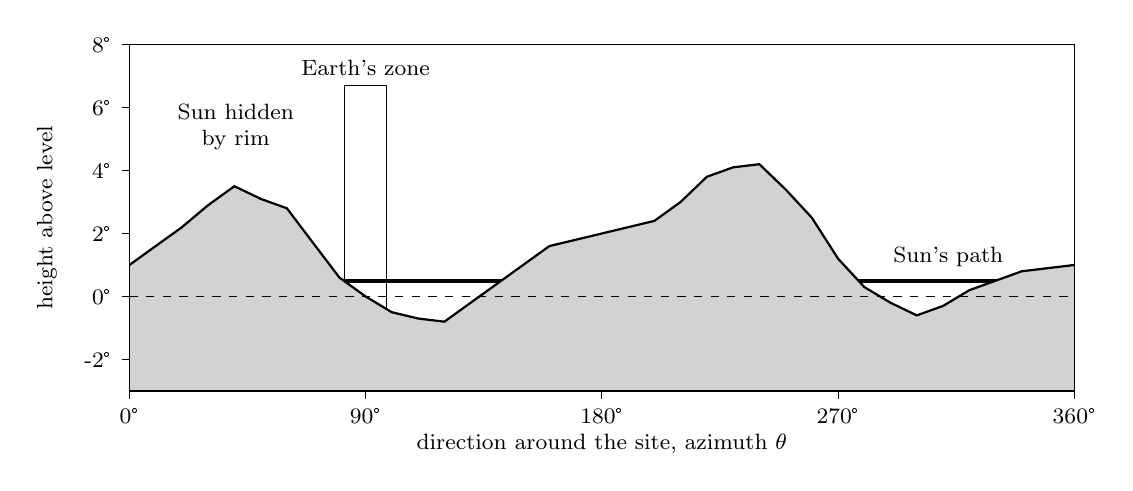
\begin{tikzpicture}[font=\footnotesize]
  \draw[fill=white] (2.733,-1.2) rectangle (3.267,2.68);
  \draw[line width=1.6pt] (0,0.2) -- (12,0.2);
  \fill[gray!35] (0,-1.2) -- (0.000,0.400) -- (0.333,0.640) -- (0.667,0.880) -- (1.000,1.160) -- (1.333,1.400) -- (1.667,1.240) -- (2.000,1.120) -- (2.333,0.680) -- (2.667,0.240) -- (3.000,0.000) -- (3.333,-0.200) -- (3.667,-0.280) -- (4.000,-0.320) -- (4.333,-0.080) -- (4.667,0.160) -- (5.000,0.400) -- (5.333,0.640) -- (5.667,0.720) -- (6.000,0.800) -- (6.333,0.880) -- (6.667,0.960) -- (7.000,1.200) -- (7.333,1.520) -- (7.667,1.640) -- (8.000,1.680) -- (8.333,1.360) -- (8.667,1.000) -- (9.000,0.480) -- (9.333,0.120) -- (9.667,-0.080) -- (10.000,-0.240) -- (10.333,-0.120) -- (10.667,0.080) -- (11.000,0.200) -- (11.333,0.320) -- (11.667,0.360) -- (12.000,0.400) -- (12,-1.2) -- cycle;
  \draw[thick] (0.000,0.400) -- (0.333,0.640) -- (0.667,0.880) -- (1.000,1.160) -- (1.333,1.400) -- (1.667,1.240) -- (2.000,1.120) -- (2.333,0.680) -- (2.667,0.240) -- (3.000,0.000) -- (3.333,-0.200) -- (3.667,-0.280) -- (4.000,-0.320) -- (4.333,-0.080) -- (4.667,0.160) -- (5.000,0.400) -- (5.333,0.640) -- (5.667,0.720) -- (6.000,0.800) -- (6.333,0.880) -- (6.667,0.960) -- (7.000,1.200) -- (7.333,1.520) -- (7.667,1.640) -- (8.000,1.680) -- (8.333,1.360) -- (8.667,1.000) -- (9.000,0.480) -- (9.333,0.120) -- (9.667,-0.080) -- (10.000,-0.240) -- (10.333,-0.120) -- (10.667,0.080) -- (11.000,0.200) -- (11.333,0.320) -- (11.667,0.360) -- (12.000,0.400);
  \draw[dashed] (0,0) -- (12,0);
  \draw (0,-1.2) rectangle (12,3.2);
  \foreach \x/\l in {0/0,3/90,6/180,9/270,12/360} \draw (\x,-1.2) -- (\x,-1.3) node[below] {\l\textdegree};
  \foreach \e in {-2,0,2,4,6,8} \draw (0,{0.4*\e}) -- (-0.1,{0.4*\e}) node[left] {\e\textdegree};
  \node[below=12pt] at (6,-1.2) {direction around the site, azimuth $\theta$};
  \node[rotate=90] at (-1.05,1.0) {height above level};
  \node[above] at (3,2.68) {Earth's zone};
  \node[above] at (10.4,0.25) {Sun's path};
  \node[align=center] at (1.35,2.15) {Sun hidden\\by rim};
\end{tikzpicture}
\caption{Steps 2 and 3 in one picture (illustrative terrain). Gray is the horizon profile from Step~1. The Sun moves along the flat line and is visible only where the line is above the gray. Earth stays inside the narrow band around 90\textdegree{} (toward longitude 0) and moves up and down; it is visible when it rises above the gray there.}
\label{fig:mask}
\end{figure}

% ---------------------------------------------------------------------
\section{Step 3: Visibility Each Hour}

For each site and hour $t$, compare the sky positions with the horizon. $H$ is interpolated between neighbouring directions (0.25\textdegree{} apart). The Sun and Earth are discs, not points (radius $r_\sun \approx 0.27^\circ$, $r_\earth \approx 0.95^\circ$ as seen from the Moon):
\begin{align}
s(t) &= \operatorname{clamp}\!\left( \frac{\mathrm{el}_\sun(t) - H(\mathrm{az}_\sun(t)) + r_\sun}{2\,r_\sun},\; 0,\; 1 \right)
&& \text{fraction of the Sun visible (power)} \\
e(t) &= \big[\, \mathrm{el}_\earth(t) + r_\earth > H(\mathrm{az}_\earth(t)) \,\big]
&& \text{any part of Earth visible (comms)} \\
b(t) &= \big[\, s(t) > 0.5 \,\big] \wedge e(t)
&& \text{power and comms together}
\end{align}

The ``any part of Earth'' rule matches the one NASA uses for its Earth-visibility maps~\cite{pgda}. Figure~\ref{fig:timeline} shows what Step~3 produces for one site.

\begin{figure}[ht]
\centering
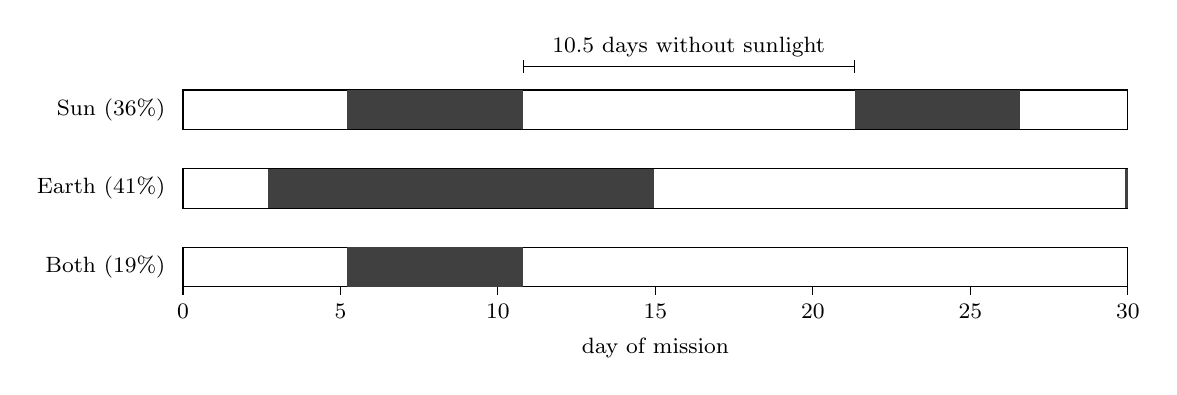
\begin{tikzpicture}[font=\footnotesize]
  \foreach \y in {0,1,2} \draw (0,{\y-0.25}) rectangle (12,{\y+0.25});
  \fill[black!75] (2.084,1.75) rectangle (4.316,2.25);
  \fill[black!75] (8.532,1.75) rectangle (10.632,2.25);
  \fill[black!75] (1.084,0.75) rectangle (5.984,1.25);
  \fill[black!75] (11.968,0.75) rectangle (12.000,1.25);
  \fill[black!75] (2.084,-0.25) rectangle (4.316,0.25);
  \node[left] at (-0.1,2) {Sun (36\%)};
  \node[left] at (-0.1,1) {Earth (41\%)};
  \node[left] at (-0.1,0) {Both (19\%)};
  \draw[|-|] (4.316,2.55) -- node[above] {10.5 days without sunlight} (8.532,2.55);
  \foreach \d in {0,5,10,15,20,25,30} \draw ({0.4*\d},-0.25) -- ({0.4*\d},-0.35) node[below] {\d};
  \node[below=12pt] at (6,-0.35) {day of mission};
\end{tikzpicture}
\caption{Step 3 output for one site over 30 days (illustrative). Black means visible. Sun and Earth are each visible about 40\% of the time, but both together only 19\%, and there is a 10.5-day stretch without sunlight that the battery must survive. A monthly average hides all of this.}
\label{fig:timeline}
\end{figure}

% ---------------------------------------------------------------------
\section{Step 4: Score and Rank}

\textbf{Gates.} A site must be within 6\textdegree{} of the pole and have a slope under 10\textdegree. Sites that fail are removed, not scored.

\textbf{Metrics over the mission window $T$.} $f_\text{sun}$, $f_\text{earth}$ and $f_\text{both}$ are the fractions of hours with $s>0.5$, $e$ and $b$ true. $g$ is the longest stretch without sunlight.
\begin{equation}
S = w_1 f_\text{sun} + w_2 f_\text{earth} + w_3 f_\text{both} - w_4\, g/T
\end{equation}
The weights are set by the user in the web app.

\textbf{Battery survival.} A simple energy budget with panel power $P_\text{panel}$, load $P_\text{load}$ and time step $\Delta t$:
\begin{equation}
E_{t+1} = \min\!\big(E_{\max},\; E_t + (P_\text{panel}\, s(t) - P_\text{load})\,\Delta t\big)
\end{equation}
The site survives if $E_t \ge E_{\min}$ at every hour. Sites that do not survive are ranked last.

\textbf{Landing accuracy.} A lander cannot hit an exact pixel; NASA's reference is within 100\,m of the target~\cite{nasa-artemis}. So rank each site by the worst score within 100\,m of it:
\begin{equation}
S_\text{robust}(p) = \min_{|q - p| \le 100\ \text{m}} S(q)
\end{equation}

\textbf{Mast height.} Using the horizons from Step~1 at several mast heights, report the lowest mast that meets the targets.

\textbf{When to land.} Repeat the scoring for every possible start date. The result is a calendar showing the best arrival dates for each site.

% ---------------------------------------------------------------------
\section{Step 5: Prove It Is Right}

\begin{enumerate}
  \item \textbf{Smooth-Moon test.} On a perfectly smooth sphere, an observer at height $h$ must see the same horizon in every direction: $H = -\arccos\!\big(R/(R+h)\big)$, about $-0.087^\circ$ for $h = 2$\,m. This also checks that $D_{\max}$ reaches past the tangent distance $\sqrt{2Rh} \approx 2.6$\,km.
  \item \textbf{Single-cone test.} One cone-shaped peak of height $P$ at distance $L$ must give exactly the angle of Equation~\eqref{eq:horizon} for $z = P$, $d = L$ in its direction, blocked at exactly $L$.
  \item \textbf{Settings by convergence.} Make every setting finer until the answer stops changing. The rule: every site's skyline stays within 0.02\textdegree{} of the finest settings in 99\% of its directions, and its Sun and Earth visibility within 0.1 percentage point. On the 240\,m map we tested the rim site plus 500 random sites within 6\textdegree{} of the pole; on 20\,m terrain, the rim site plus 150 random sites within 13\,km of the pole. Results:
  \begin{itemize}
    \item Look-out distance $D_{\max} = 250$\,km. At 200\,km, whole sectors of some sites are still 0.49\textdegree{} off; beyond 250\,km nothing changes.
    \item 1{,}440 directions. With 360 directions, the worst site is 0.058\textdegree{} off.
    \item Step factor 0.002: far from the site, each step is 0.2\% of the distance.
    \item 20\,m terrain out to 40\,km. At 20\,km, sectors are 0.044\textdegree{} off.
  \end{itemize}
  \item \textbf{Compare with NASA's maps.} NASA's illumination maps~\cite{pgda} are long-term averages, so compare them with our results averaged over at least a year, not one month. Done at Shackleton's rim: we ran the engine at the centres of the 100 NASA 60\,m pixels around our rim site, with 20\,m terrain nearby and 240\,m beyond. From a 2\,m mast, our rough yearly Sun estimate matches NASA's map with correlation 0.92 and an average difference under half a percentage point, with 93\% of pixels within 10 points. Always compare at pixel centres, never ``NASA's value at the site'': a site can sit exactly on the corner of four NASA pixels (at our rim site they read 0\%, 6\%, 47\% and 56\%).
  \item \textbf{Check the sky.} The Sun stays within about $\pm1.5^\circ$ of level and Earth within about $\pm6.7^\circ$ (Step~2).
\end{enumerate}

% ---------------------------------------------------------------------
\section{Files Passed Between Steps}

Everyone builds against fake files in these formats from day one, so nobody waits for anyone. Angles are in degrees, times are hourly UTC, and azimuth follows the convention in Step~0.

\begin{table}[H]
\centering
\renewcommand{\arraystretch}{1.2}
{\small\setlength{\tabcolsep}{4pt}%
\begin{tabularx}{\textwidth}{l Y l l l}
\toprule
\textbf{File} & \textbf{Contents} & \textbf{Shape} & \textbf{Made by} & \textbf{Used by} \\
\midrule
\texttt{dem.npy} & Terrain heights (m) on the map grid & rows $\times$ cols & Step 0 & Step 1 \\
\texttt{sites.csv} & id, $x$, $y$, lat, lon, height, slope & one row per site & Step 0 & Steps 1, 4 \\
\texttt{horizon.npy} & Horizon profile per site and mast height & sites $\times$ masts $\times$ 1440 & Step 1 & Step 3 \\
\texttt{blocker.npy} & Distance to the terrain that sets the horizon (m) & sites $\times$ masts $\times$ 1440 & Step 1 & Step 3, web app \\
\texttt{complete.npy} & True where the walk reached $D_{\max}$ on the map & sites $\times$ masts $\times$ 1440 & Step 1 & Step 3 \\
\texttt{horizon\_meta.json} & Settings: directions, convention, masts, $D_{\max}$, step factor, $R$, terrain files & --- & Step 1 & Step 3 \\
\texttt{sky.npz} & Sun and Earth az/el each hour & sites $\times$ hours & Step 2 & Step 3 \\
\texttt{visibility.npz} & $s(t)$, $e(t)$, $b(t)$ & sites $\times$ hours & Step 3 & Step 4 \\
\texttt{results.json} & Scores, metrics, timelines of top sites & per site & Step 4 & Web app \\
\bottomrule
\end{tabularx}}
\caption{Data contracts between steps. Read the number of directions and the mast heights from \texttt{horizon\_meta.json} instead of hard-coding them.}
\end{table}

% ---------------------------------------------------------------------
\section{Who Owns Which Step}

\begin{table}[H]
\centering
\renewcommand{\arraystretch}{1.35}
\begin{tabularx}{\textwidth}{l Y l}
\toprule
\textbf{Step} & \textbf{Role} & \textbf{Member} \\
\midrule
Step 0: terrain and sites & Terrain and sites & \rule{3cm}{0.4pt} \\
Step 1: horizon profile & Horizon engine & \rule{3cm}{0.4pt} \\
Step 2: Sun and Earth positions & Sky (SPICE) & \rule{3cm}{0.4pt} \\
Steps 3--4: visibility and scoring & Scoring and mission model (integrator) & \rule{3cm}{0.4pt} \\
Display & Web app & \rule{3cm}{0.4pt} \\
Step 5 and submission & Validation, story and submission & \rule{3cm}{0.4pt} \\
\bottomrule
\end{tabularx}
\caption{Step ownership. The horizon engine owner also writes the smooth-Moon and cone tests.}
\end{table}

% ---------------------------------------------------------------------
\section{What Makes Our Tool Different}

NASA already publishes average illumination and Earth-visibility maps~\cite{pgda}, and judges may know them. Averages cannot answer a mission's real questions, and Figure~\ref{fig:timeline} shows why. Our tool answers them for a specific mission:
\begin{itemize}
  \item When will this site have power and Earth contact \emph{at the same time}?
  \item Will a lander arriving on a given date survive its whole mission?
  \item How tall must the mast be at this site?
  \item Is the site still good if we land 100\,m off target?
  \item Which arrival date is best?
\end{itemize}

% ---------------------------------------------------------------------
\begin{thebibliography}{9}
\bibitem{nasa-artemis}
NASA, \emph{Artemis Overview, 2025 International Space Apps Challenge}, NTRS 20250009323.
\url{https://ntrs.nasa.gov/api/citations/20250009323/downloads/ArtemisOverview2025IntSPAPPSChallenge.pdf}

\bibitem{pgda}
NASA Goddard Planetary Geodesy Data Archive, \emph{Lunar Polar Illumination}.
\url{https://pgda.gsfc.nasa.gov/products/69}

\bibitem{lola}
NASA PDS Geosciences Node, \emph{LRO LOLA polar elevation maps} (LDEM\_875S\_20M, LDEM\_75S\_240M).
\url{https://pds-geosciences.wustl.edu/lro/lro-l-lola-3-rdr-v1/lrolol_1xxx/data/lola_gdr/polar/}

\bibitem{spice}
NASA NAIF, \emph{The SPICE Toolkit}.
\url{https://naif.jpl.nasa.gov/naif/}

\bibitem{spiceypy}
SpiceyPy, Python wrapper for SPICE.
\url{https://github.com/AndrewAnnex/SpiceyPy}
\end{thebibliography}

\end{document}
